%----------------------------------------------------------------------------------------
%	Hardware
%----------------------------------------------------------------------------------------

\chapter{Hardware Components}

\section{Prior Art}
There are many existing products in the market for animal weighing, however, most of them are for use in a farm setting to weigh and track heavy animals such as cows and horses. As a result, the cost of such a system is expensive since the weight capacity goes up to a few thousand kilograms, and the weighing platform must be large enough to fit the animals. The load bars in these products usually have stricter requirements, which further increases the cost. Such a product is less suitable for measuring the weights of small and medium dogs in a cost-effective manner.

One example is the AgriEID Heavy Duty Load Bar digital livestock weight system which is available for purchase at the price of \$1395. The product is enclosed in stainless steel with four different dimensions depending on the specific model, some important technical specifications are summarized in Table \ref{table:tech specs AgriEID}.

\begin{table}[h]
\centering
\begin{tabular}{|l|m{6cm}|}
    \hline
    Parameter & Value \\
    \hline
    Weight Range & 0 to 3000kg \\
    Wight Accuracy & 0.003kg \\
    Supply Voltage & 6V rechargeable battery \\
    Communication &	RS232 serial communication, optional Bluetooth/WIFI/4-20mA \\
    Weight of load bar	& 11.5kg each \\
    Display & LCD screen \\
    Operating Temperature & -10 to 40°C \\
    \hline
\end{tabular}
\caption{Technical specifiations of AgriEID.}
\label{table:tech specs AgriEID}
\end{table}

This product is capable of measuring the weight of any size or type of animal up to its maximum capacity, the display monitor has 7 functional keys allowing users to choose what they want to do. The main functionalities are date display, weight unit exchange, weight records retrieval, tare and zero. However, it requires heavy duty 5m length dual cables to connect the digital display to the load bars, exposing tripping hazard to both staff and the animals. The weighing platform does not come with the product and the company does not sell them, customers have to consult a local engineering firm and this adds an extra cost of \$500 to \$800. The Livestock Management Software stores weight measurements over time, and provides powerful data analysis and secure digital record keeping, but only the first 12 months are free.

\section{Operating Principles}
There are four load cells in the weighing platform used to measure weight. Each load cell has two strain gauges connected in series, one of them is configured to stretch and the other configured to compress under weight, which in turn changes the resistance of the strain gauges, the resistance will increase in the stretching one and decrease in the other. When current flows through the strain gauges, their resistance change is reflected by the voltage change across them, this voltage change can be measured and converted to a weight measurement according to how much the resistance changes under weight.

The four load cells are connected in a Wheatstone bridge as shown in the proposed design, there are four groups of resistors, R1 and R2, R3 and R4, R5 and R6, R7 and R8, each group belongs to one load cell. R1, R4, R5 and R8 will stretch under weight, so their resistances will increase, while R2, R3, R6 and R7 will compress under weight, so their resistances will decrease. Voltage measurement will be taken between Vsen+ and Vsen-. When there is no weight on the scale, the voltage difference between Vsen+ and Vsen- ideally should be zero, once the dogs are on the scale, the voltage at Vsen+ will drop below the voltage at Vsen-, and the voltage measured is negative, this voltage is conditioned and then fed to the input of ADC.

Since the Wheatstone bridge is powered by 3.3V and the resistance change in the strain gauges are in mili ohms under weight, the voltage difference between Vsen+ and Vsen- is very small. The ADC input can only accept voltage between 0 and 3.3V, the voltage needs to be shifted up and amplified to make it suitable for the ADC to take a reading. An operational amplifier can be used for amplifying the signal, in our proposed design, an instrumentation amplifier with a voltage offset of 1.8V and a gain of around 1200 is used to shift and amplifier the signal. Due to the output limitation of the LM358 opamp, when powered by 3.3V, the maximum voltage it can output is 1.95V. As a result, the voltage fed to the ADC input is in the range of 0.2V to 1.89V. A differential amplifier can also be used as an alternative, however, due to the configuration of resistors around it, the Wheatstone bridge will be loaded and results in an inaccurate measurement.

To stabilize the signal, two filters are added to filter unwanted noise in Vsen+ and Vsen- before feeding them to the input terminals of the instrumentation amplifier. Another output filter is added to stabilize voltage at the output of the instrumentation amplifier. Capacitors are also added in parallel to some resistors in the instrumentation amplifier.

\section{Proposed Design}
Figure \ref{fig:hardware} below shows the proposed design of our electronic circuit, divided into four functional blocks, the Wheatstone bridge, two input filters, one output filter and an instrumentation amplifier.

\begin{figure}[h]
    \centering
    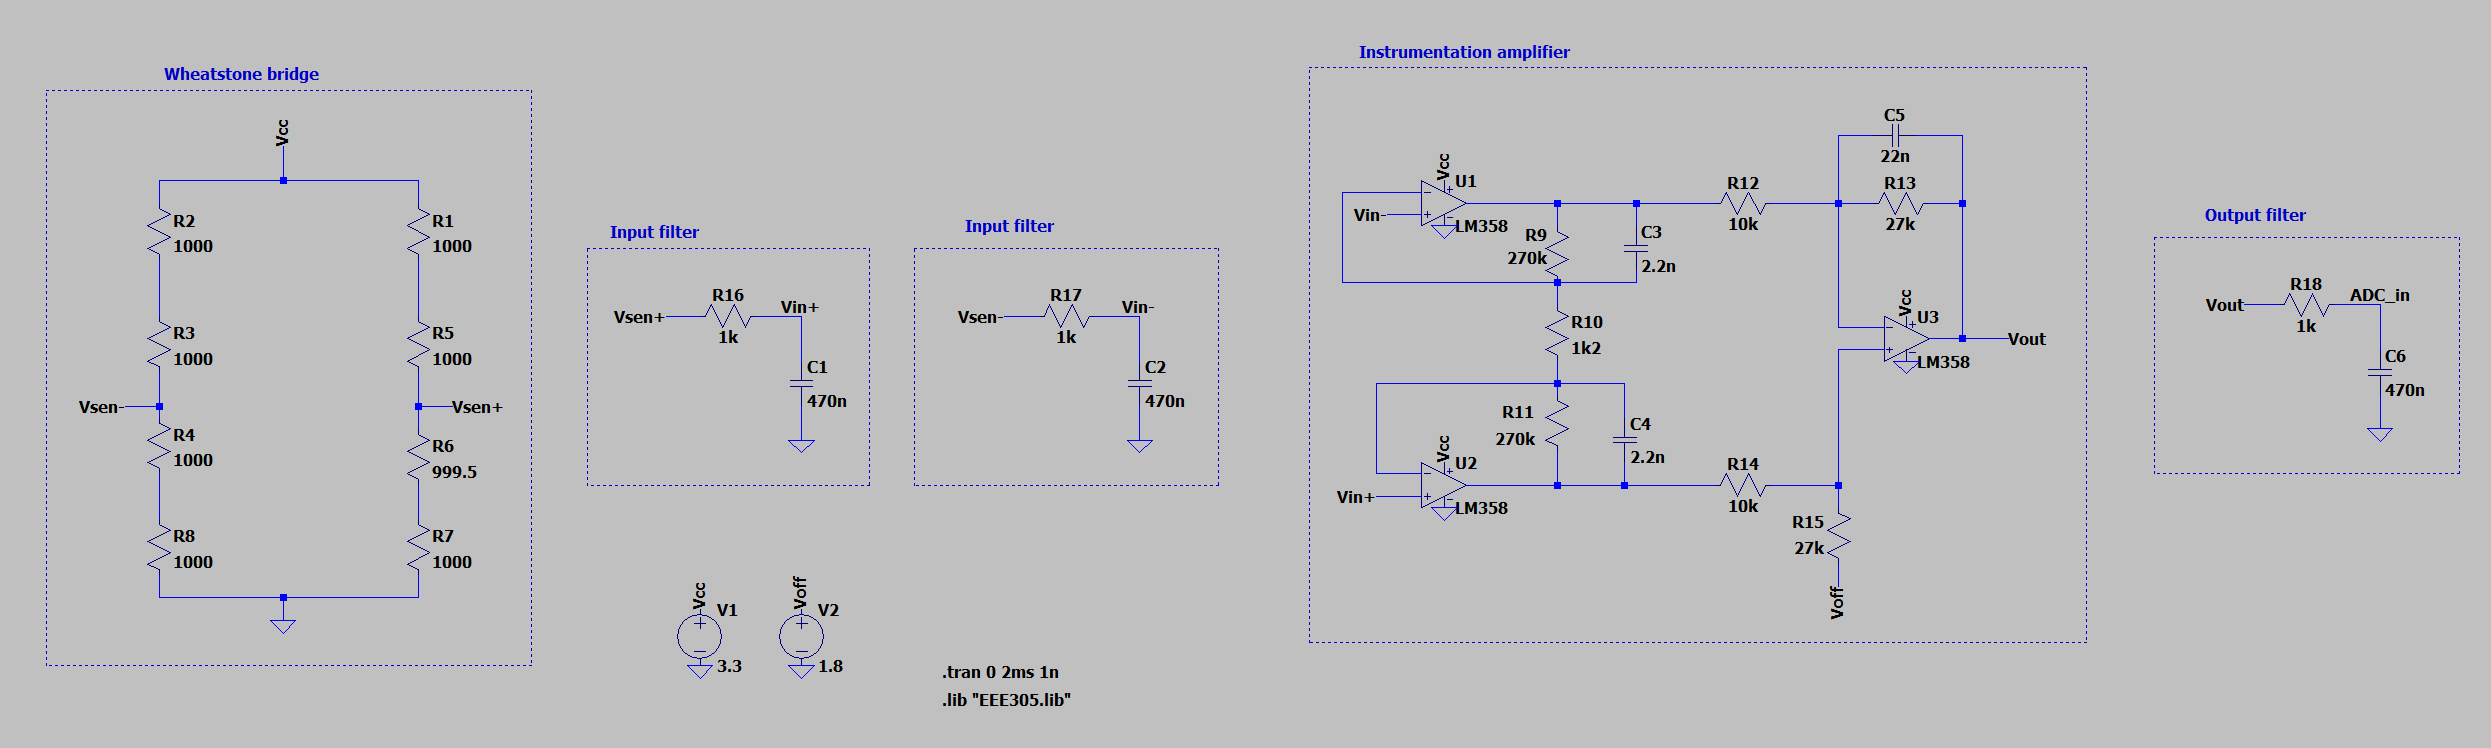
\includegraphics[width=\textwidth]{proposal/parts/hardware-circuit.png}
    \caption{Hardware design divided into functional blocks.}
    \label{fig:hardware}
\end{figure}

The scale is powered by 4 x AAA batteries, the 3.3V used to power the Wheatstone bridge and the instrumentation amplifier are derived from the battery using a linear regulator, which is not shown in Figure \ref{fig:hardware}. The 1.8V offset at the instrumentation amplifier will be derived from a voltage divider connected to the output of the linear regulator. The regulator can be turned off when no dogs are being weighed.

Four LEDs and a tare button will be added to connect to Raspberry Pi Pico W, the LEDs are used for indicating successful weight measurement, WiFi connection, power and tare respectively. as well as adding a tare function to our product.

The technical specifications of the proposed design are summarized in Table \ref{table:tech specs}.

\begin{table}[h]
\begin{center}
\begin{tabular}{|l|l|}
    \hline
    Parameter & Value \\
    \hline
    Weight Range & 0 to 25kg \\
    Weight Accuracy & 0.25kg \\
    Supply Voltage & 4 x AAA Batteries \\
    Output Voltage Range & 0.2 to 1.89V \\
    Operating Temperature & 0 to 40°C \\
    Display & LED indicates a successful reading \\
    Compliance & RoHS and WEEE (AS/NZS 5377) \\
    \hline
\end{tabular}
\caption{Technical specifications of the proposed design.}
\label{table:tech specs}
\end{center}
\end{table}

The proposed hardware circuit can accurately measure weight between 0 to 25kg, in steps of 0.25kg. The circuit is drawn and verified in LTspice, with simulation results summarised in Table \ref{table:simulation}. Screenshots of simulation results could be found in Appendix C. The expected component cost is \$9.33 with the Bill Of Materials included in Appendix D.

\begin{table}[h]
    \begin{center}
    \begin{tabular}{|l|l|}
        \hline
        Voltage input & Voltage output \\
        \hline
        0mV & 1.799V \\
        -0.206mV & 1.549V \\
        -0.412mV & 1.299V \\
        -0.619mV & 1.043V \\
        -0.825mV & 0.799V \\
        -1.032mV & 0.549V \\
        -1.238mV & 0.299V \\
        \hline
    \end{tabular}
    \caption{Simulation results.}
    \label{table:simulation}
    \end{center}
\end{table}
